% Appendix A

\chapter{Feedforward Neural Networks} % Main appendix title

\label{AppendixA} % For referencing this appendix elsewhere, use \ref{AppendixA}

\textcolor{red} {[TODO: Introduce FFNs for discrete signals] }

\section{Terminology}

Figure~\ref{fig:Terminology} presents the terminology in a FNN with three input signals, a hidden layer with two neurons, and one output signal.

\begin{figure}[h]
	\centering
	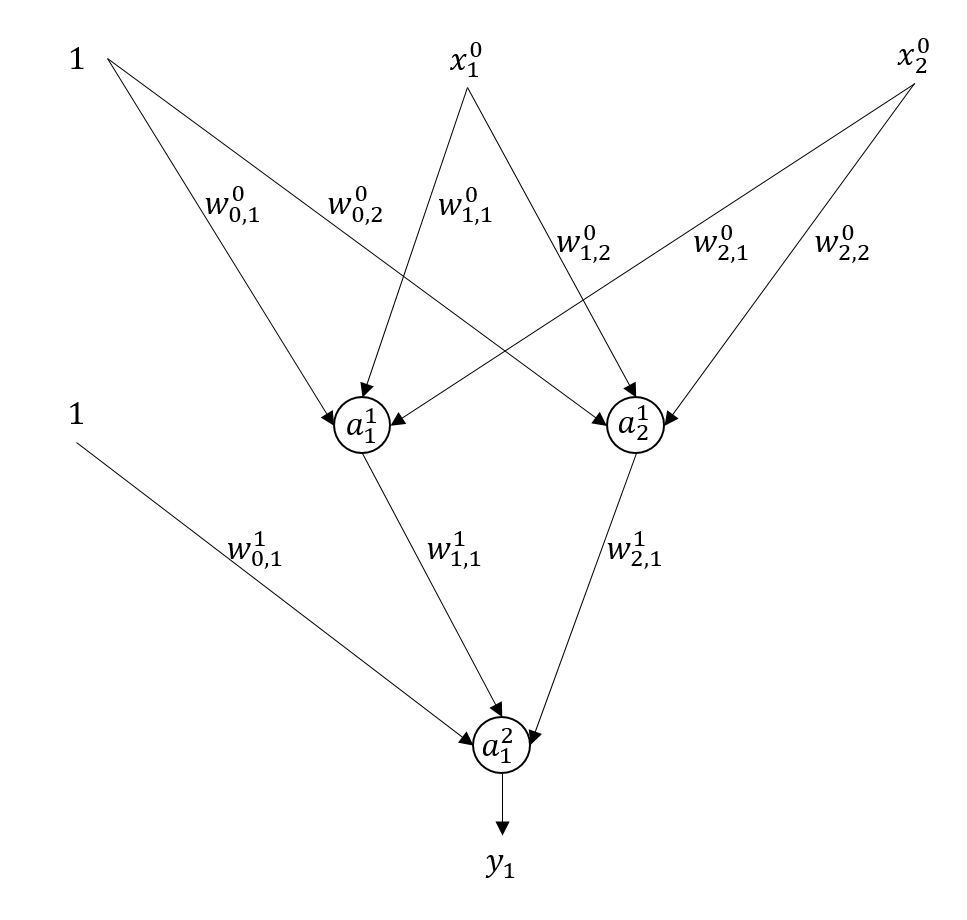
\includegraphics{Figures/ffn_v1.PNG}
	\decoRule
	\caption[Neural Networks Terminology]{Neural Networks Terminology}
	\label{fig:Terminology}
\end{figure} 


In this figure $w^{m}_{ij}$ represents the weight in the synaptic link that joins neuron $a^{m}_{i}$ with neuron $a^{m+1}_{j}$. Also $m$ indicates the layer in the neural network, where the input layer has $m=0$, and the output layer $m=2$. The two input signals are given by $x^{0}_{1}, x^{0}_{2}$, and the output signal by $y_1$. Even though it is not shown in the figure, the output of the hidden neurons  $a^{1}_{1}$ and $a^{1}_{2}$ are $x^{1}_{1}$ and $x^{1}_{2}$ respectively.

\section{Backpropagation Training in FNNs}
Supervised training of FNNs can be done through the backpropagation method, which consists in propagating the output error with respect to the training data down all the internal layers in the network in order to adjust the weights while optimizing a model. The enumeration below presents the steps of a pseudo algorithm that implements backpropagation training in a FNN. Each of these steps is further explained in the remaining of this section.

	\begin{enumerate}\label{enum:A1}
	\item[\textbf{Step 1}] Initialize parameters in Neural Network
	\item[\textbf{Step 2}] Perform Forward Pass
	\item[\textbf{Step 3}] Compute Error
	\item[\textbf{Step 4}] Update link Weights
	\item[\textbf{Step 5}] Repeat Steps 2 to 4 until reducing Error to target value
	\end{enumerate}


\subsection{Initialization and Forward Pass}
The weights in a neural network are initialized randomly, typically to small values. 
\\
Forward pass is the process through which a neural network is triggered with a given input signal to activate internal and output neurons. 
\\
\textcolor{red} {[TODO: Expand on forward pass and initialization of parameters] }

\subsection{Error Computation}
The error represents the difference between the predicted output $y^*$ calculated in forward pass, and the real output $y$ which is given as part of the training data. The MSE function \ref{eq:A1} is commonly use to measure these errors between predicted and real output for a training data set with $n$ samples.

\begin{equation}\label{eq:A1}
E= \sum_{i=1}^{n} E_i =\frac{1}{2}\sum_{i=1}^{n}(y_i^* - y_i)^2
\end{equation}

\subsection{Weigths Optimization}
The weights in a neural network represent the trainable parameters, and their optimization requires the calculation of the error gradient with respect to each of the weights $\frac{\partial E}{\partial w_{i,j}}$. The weigthts in each layer are adjusted through gradient steps in order to approach a minimum solution of the error function. Function \ref{eq:A2} shows the gradient step calculation to update a weight, where $\gamma$ is the learning rate.

\begin{equation}\label{eq:A2}
	w^{new}_{i,j} = w_{i,j} - \gamma \frac{\partial E}{\partial w_{i,j}}
\end{equation}

\subsubsection{Error Gradient Computation}
The computation of the gradients is performed first with respect to the weights that connect to the output layer, and then backpropagates down the neural network until reaching the weights that connect to the input layer. Equation \ref{eq:A3} shows a generalization of the error gradient with respect to weights $w^{M-1}_{i,j}$ of the synaptic links that connect to the output neuron $a^{M}_{1}$, where $M$ is the total number of layers in a neural network.

\begin{equation}\label{eq:A3}
\frac{\partial E_i}{\partial w^{M}_{i,j}} = \frac{\partial}{\partial w^{M}_{i,j}} \frac{1}{2}(y_i^* - y_i)^2 = (y_i^* - y_i)\frac{\partial}{\partial w^{M}_{i,j}} (\sigma(W^{M}_{i,j} X^{M-1}_i) - y_i)
\end{equation}

\textcolor{red} {[TODO: Keep Expanding on backpropagation training ] }




